\documentclass[a4paper,man,biblatex]{apa6}
\usepackage[american]{babel}
\usepackage{csquotes}
\usepackage[backend=biber]{biblatex}
\usepackage[document]{ragged2e}
\setlength{\RaggedRightParindent}{0.5in}
\addbibresource{references.bib}
\usepackage{graphicx}
\usepackage{url}
\usepackage{xpatch}
\xpatchbibdriver{online}
  {\printfield{entrysubtype}}
  {\printfield{entrysubtype}%
   \newunit\newblock
   \printfield{note}}
  {}
  {}

\renewcommand{\abstract}[1]{}

\title{Inquiry Log \#1}
\shorttitle{Sleep Data Analysis}
\author{Armant Touche}
\affiliation{Portland State University}
\date{\today}

\begin{document}
\thispagestyle{otherpage}
\setcounter{biburllcpenalty}{7000}
\setcounter{biburlucpenalty}{8000}

%\maketitle

\noindent Name: Armant Touche\newline
\noindent Date: 4/22/2020

\subsection{Results}

After recording my sleep times and hours slept, I was not surprised I slept alot. I've read books and materials that highlight the link between memory and sleep, specifically how much sleep is beneficial for memory consolidation. Memory consolidation from my understanding involves either short-term or long-term crystallization so if you were in school and you studied consistently then it is important to recieve good quality sleep. Noting that people require different amounts of sleep. I require a lot of sleep because if I do not, I become lethargic and can become easily distracted. I spent most of my time in the military in this state-of-thought because that was the nature of my job. After getting out of the military, I decided to implement what I knew I needed which was large amount of sleep. On average, I sleep about nine hours each night and I've noticed the benefits. I am normally in a better mood and I find that consistent studying, which is normally around $1-1.5$ hours per subject each day. My good grades are result of that, not trying to boast but am trying to prove the point that you can study less each day and potentially make better grades. The motivation for getting better sleep is I have to study less about a subject because I can experience effective memory consolidation during my sleep which aides both short-term and long-term crystallazition.

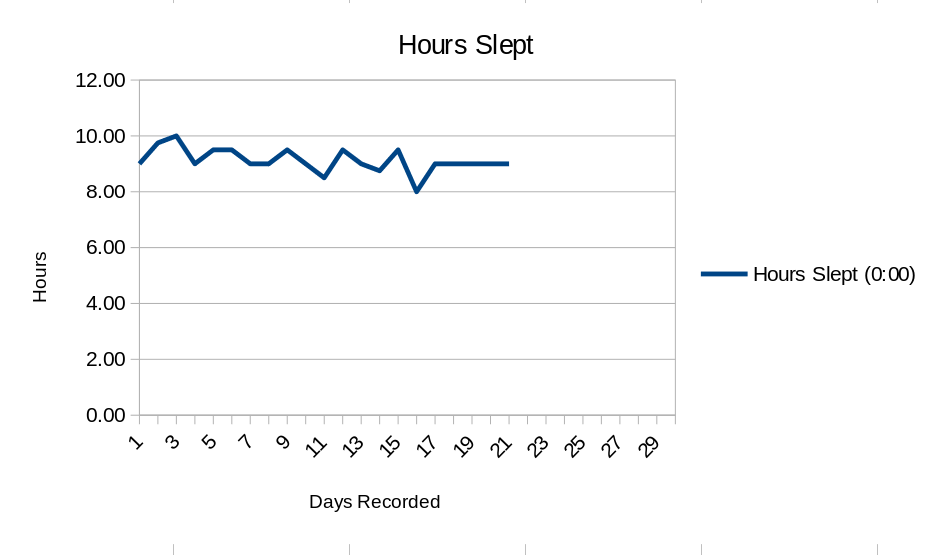
\includegraphics[width=.75\linewidth]{hours_slept}

\subsection{Conclusion} There is a lot of literature on sleep hygiene especially studies on college students and how they practice sleep hygiene. The stereotype of a traditional college student sleep habits are known to not be that great. Pulling all-nighter's for an exam or after a long week of classes, instead of resting over the weekend, students tend to party hard. I used to fit that stereotype and I am not surprised that I had difficulties with school. I could remeber getting around $5-6$ hours of sleep and also going to parties of all sorts. These added stressors along with normal stressors every adults experiences really started to take a toll on me physically and mentally. Relfecting back on my old ways, I am glad I made the choice to better myself and sleep was one of the choices I made. I think sleep hygiene should be taught earlier than what \textit{Behavioral Medicine}'s article suggested \autocite{sleep101}. Reason being is that a lot of bad habits are learned in the high school. Outside of sleep hygiene, alcohol and study habits are some other learned, bad habits from high school which is another subject I will not get into. Overall I agree with alot of what \textit{Behavioral Medicine}'s article had to say. College students with poor sleep patterns have an overall lower quality of life.

\printbibliography

\end{document}
